\documentclass[a4paper]{ltjsarticle}

\usepackage[dvipdfmx]{graphicx}
\usepackage[dvipdfmx,hidelinks,pdfusetitle]{hyperref}
\hypersetup{
    colorlinks=false,
    bookmarksnumbered=true,
    pdfborder={0 0 0},
    bookmarkstype=toc
}
\usepackage[nobreak]{cite}
\usepackage{pxjahyper}
\usepackage{amsmath}
\usepackage{tikz}

\usetikzlibrary{datavisualization}
\usetikzlibrary{positioning}
\usetikzlibrary{shapes.geometric, shapes.misc}
\usetikzlibrary{patterns}
\usetikzlibrary{calc}

\begin{document}

\begin{itembox}[l]{京都大学 2013年 第5問}
    $xy$ 平面内で,$y$ 軸上の点Pを中心とする円 $C$ が2つの曲線

    \begin{equation*}
        C_1\colon y=\sqrt{3}\log (1+x), C_2\colon y=\sqrt{3}\log (1-x)
    \end{equation*}

    とそれぞれ点A,点Bで接しているとする。さらに $\triangle\mathrm{PAB}$ はAとBが $y$ 軸に関して対称な位置にある正三角形であるとする。このとき3つの曲線 $C, C_1, C_2$ で囲まれた部分の面積を求めよ。ただし,2つの曲線がある点で接するとは,その点を共有し,さらにその点において共通の接線を持つことである。
\end{itembox}

\begin{figure}[!ht]
    \centering
    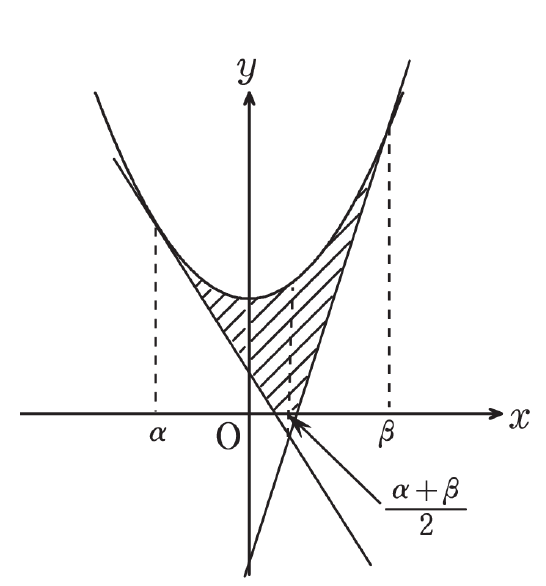
\includegraphics[width=0.5\textwidth]{f1.png}
\end{figure}

$C$ と $C_1$ は点Aで接するから,Aにおける $C$ と $C_1$ の接線は一致する。この接線を $t$ とする。ここで,$\triangle\mathrm{OAB}$ は $y$ 軸に関して対称な正三角形であるから,直線APの傾きは $-\sqrt{3}$ 。したがって, $t$ の傾きは $1/\sqrt{3}$ 。また,$C_1$ について $y'=\sqrt{3}/(1+x)$ であるから,Aの $x$ 座標を $t$ とすると,

\begin{equation*}
    \frac{\sqrt{3}}{1+t}=\frac{1}{\sqrt{3}}\quad\Longleftrightarrow\quad t=2
\end{equation*}

よって,$\mathrm{A}(2, \sqrt{3}\log 3)$ である。さらに,$\mathrm{PA}=\mathrm{AB}=2t=4$ であり,$\mathrm{OP}=\sqrt{3}\log 3+2\sqrt{3}$

また,円 $C$ と $y$ 軸の交点のうち,$y$ 座標が小さい方をQとする。$C$,$C_1$,$C_2$ で囲まれた図形は図の斜線部分であり,$y$ 軸に対して対称である。面積を $S$ とし,$\mathrm{H}(2, 0)$ とすると,

\begin{equation*}
    S=2\left\{(\text{台形OHAPの面積}S_1)-(\text{扇形PAQの面積}S_2)-\int_0^2\sqrt{3}\log(1+x)dx\right\}
\end{equation*}

ここに,

\begin{align*}
    S_1                         & =\frac{1}{2}\left\{(\sqrt{3}\log 3+2\sqrt{3})+\sqrt{3}\log 3\right\}\times 2=2\sqrt{3}\log 3+2\sqrt{3} \\
    S_2                         & =\frac{1}{2}\mathrm{PA}^2\cdot\frac{\pi}{6}=\frac{4}{3}\pi                                             \\
    \int_0^2\sqrt{3}\log(1+x)dx & =\sqrt{3}\Bigl[(1+x)\log(1+x)\Bigr]_0^2=\sqrt{3}(3\log 3-2)
\end{align*}

以上より,

\begin{align*}
    S & =2\left\{(2\sqrt{3}\log 3+2\sqrt{3})-\frac{4}{3}\pi-\sqrt{3}(3\log 3-2)\right\} \\
      & =8\sqrt{3}-2\sqrt{3}\log 3-\frac{8}{3}\pi
\end{align*}

\end{document}
